\documentclass[a4paper,10pt]{book}

\usepackage[pdftex]{graphicx}
\usepackage{html}

\title{Juicer - User Manual\\\includegraphics{../juicer-new.png}}

\begin{document}

\maketitle


\section{The Main Window}

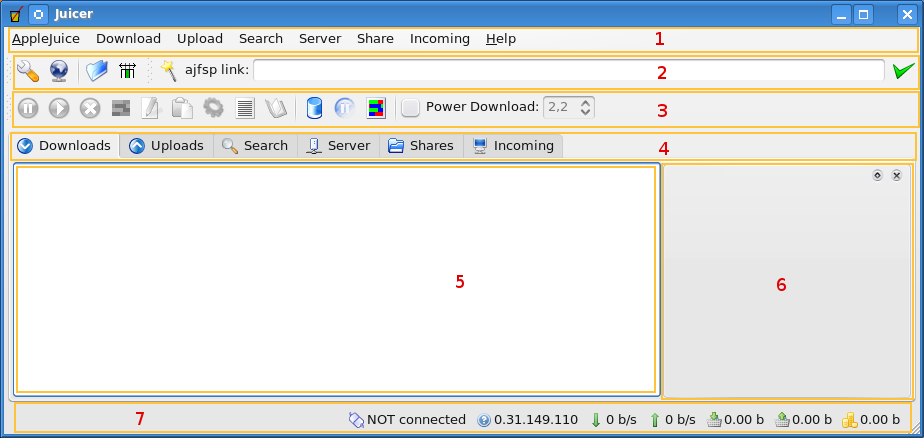
\includegraphics[width=1.0\textwidth]{./images/mainwindow.png}


\begin{enumerate}
 \item Menu Bar: general and specific menus for the modules
 \item General Tool Bar: tool bar wit general, module independent actions\\
 \begin{itemize}
  \item 
\includegraphics[width=22px]{../configure.png} opens the options dialog where you can configure Juicer as well as the appleJuice core
  \item 
\includegraphics[width=22px]{../network.png} show information of the appleJuice network
  \item 
\includegraphics[width=22px]{../fileopen.png} opens a link list file and adds all links in it
  \item 
\includegraphics[width=22px]{../show_table_column.png} adjusts the width of all columns of the currently visible tree view
  \item 
\includegraphics[width=22px]{../wizard.png} adds all links that are currently in the clipboard
  \item 
\includegraphics[width=22px]{../button_ok.png} adds the link of the input field
 \end{itemize}
 \item Module Tool Bar: tool bar with actions of the selected module, changes if another module was selected
 \item Tab Bar: module selection\\Juicer consists of several modules whereas the data of each is shown in its very own tab in the main window (5). There are six different modules:\\
 \begin{itemize}
  \item \htmlref{
\includegraphics[width=16px]{../small/downloads.png}}{sec:downloads} \htmlref{Downloads}{sec:downloads}
  \item \htmlref{
\includegraphics[width=16px]{../small/uploads.png}}{sec:uploads} \htmlref{Uploads}{sec:uploads}
  \item \htmlref{
\includegraphics[width=16px]{../small/viewmag.png}}{sec:search} \htmlref{Search}{sec:search}
  \item \htmlref{
\includegraphics[width=16px]{../small/server.png}}{sec:server} \htmlref{Server}{sec:server}
  \item \htmlref{
\includegraphics[width=16px]{../small/folder_open.png}}{sec:shares} \htmlref{Shares}{sec:shares}
  \item \htmlref{
\includegraphics[width=16px]{../small/network_local.png}}{sec:incoming} \htmlref{Incoming}{sec:incoming}
 \end{itemize}
 \item Tab Widget: module content
 \item Dock Widget: shows some extra information like the part list of a download; you can move, release, and hide it
 \item Status Bar: general status information
 \begin{itemize}
  \item 
\includegraphics[width=16px]{../small/connect_established.png} since when the core is connected to a server
  \item 
\includegraphics[width=16px]{../small/help.png} the version of the core
  \item 
\includegraphics[width=16px]{../small/arrow_down.png} speed of all downloads
  \item 
\includegraphics[width=16px]{../small/arrow_up.png} speed of all uploads
  \item 
\includegraphics[width=16px]{../small/basket_put.png} amount of data downloaded since the core is running
  \item 
\includegraphics[width=16px]{../small/basket_remove.png} amount of data uploaded since the core is running
  \item 
\includegraphics[width=16px]{../small/coins.png} amount of credits available
 \end{itemize}

\end{enumerate}

%  \item \includegraphics{../.png} 


\subsection{Downloads}
\label{sec:downloads}
The Downloads module is obviously the most important part of Juicer and therefor provides the most amount of information.
Every download is shown by one line in the tree view that can be expanded by clikcing on the little plus sign or by double clicking
the row in order to show the users where you are downloading from or may download from. They are sorted by status:
\begin{enumerate}
 \item "active": meaning you are currently getting data from it
 \item "queueing": you are in the queue of an user and you may download from it if you wait or increase your power download
 \item "other": you are not acutally connected to these users by different reasons
\end{enumerate}
You can manipulate downloads by selecting them and clicking on a button in the toolbar or in the context menu.
\begin{itemize}
 \item \includegraphics[width=22px]{../.png} pauses the selected download(s)
 \item \includegraphics[width=22px]{../.png} starts the selected download(s)
 \item \includegraphics[width=22px]{../.png} cancels the selected download(s)
 \item \includegraphics[width=22px]{../.png} shows the part list of the selected download(s) in a separate window
 \item \includegraphics[width=22px]{../.png} changes the file name on the selected download(s)
 \item \includegraphics[width=22px]{../.png} changes the filename(s) of the selected download(s) by the content of the clipboard; this operation preserves file suffixes and adds "_1", "_2", ... in front of the file suffix if multiple downloads are selected
 \item \includegraphics[width=22px]{../.png} opens the selected download(s) with the application defined in the configuration
 \item \includegraphics[width=22px]{../.png} changes the target folder of the selected download(s)
 \item \includegraphics[width=22px]{../.png} copies the ajfsp link(s) of the selected download(s) into the clipboard
 \item \includegraphics[width=22px]{../.png} creates a link list of ajfsp links of the selected download(s) and writes them to a file
\end{itemize}

Additionally there are operation that infect downloads or the download view in general:
\begin{itemize}
 \item \includegraphics[width=22px]{../.png} removes finished and canceld downloads from the list
 \item \includegraphics[width=22px]{../.png} hides (NOT removes) puased downloads
 \item \includegraphics[width=22px]{../.png} enables/disabled the dock widget with the part list
\end{itemize}

\subsection{Uploads}
\label{sec:uploads}

\subsection{Search}
\label{sec:search}

\subsection{Server}
\label{sec:server}

\subsection{Shares}
\label{sec:shares}

\subsection{Incoming}
\label{sec:incoming}

\section{The Configuration}


\end{document}
